% % CHAPITRE 1 : SYNTHESE BIBLIO
%
%Réflexions
%
%NE PAS OUBLIER DE CALER UN MAXIMUM D'ORDRE DE GRANDEUR ! 
%	(émissions CO2, CH4, stocks flux, surface des tourbières, végétation ...)
%
%Bien différencier l'intro générale qui doit être lisible par un béotien, de l'intro au travail de la thèse qui doit être un état de l'art précis et documenté sur les travaux antérieurs (synthèse biblio)
%
%Ou caler la partie de biblio sur l'expérimentation ... (peut être dans la synthèse biblio, paragraphe "approche mise en oeuvre"
%INTRODUCTION GENERALE (à mettre dans le chapitre Intro)
%
%- Qu'est ce qu'une tourbière ? (Éventuellememt comment se forme-t-elle ?)
%	*Définition
%	*Formation/Évolution (stockage du C, battement de la nappe ?)
%	*Classification
%- Les tourbières et les hommes 
%	*Usages d'hier et d'aujourd'hui (Combustible, horticulture, matériau de construction)
%	*Les thématiques scientifiques (pourquoi les avoir étudier et les étudier en gros)
%	*Le contexte dans lequel va s'inscrire le travail qui suit
%
%SYNTHESE BIBLIOGRAPHIQUE
%
%- Quelles sont les grandes thématiques de recherche liées aux tourbières ?
%	*Exploitation
%	*Archives
%	*Émissions de GES
%- Plus précisément quelles sont les grands axes de recherche sur ces écosystèmes et liés aux émissions de GES.
%	*Processus de création de GES (CO2 et CH4) (Facteurs contrôlant généralement invoqués)
%	*Processus de migration des GES dans le profil
%	*Processus de stockage/capture
%- Approches mise en oeuvre
%	*Modélisation (empirique et mécaniste)
%	*Expérimentation (différentes techniques pour mesurer les émissions de GES, différentes techniques de chambre...)
%	*Variabilité spatio-temporelle (notion d'échelle)
%	
%	DOIS-JE TRAITER
%	La classification des tourbières ?
%	Hummock and Hollow ? Dire qu'on n'est pas dans ce niveau de détail ?
%	
%
%HISTORIQUE (études concernant les tourbières)
%
%1968-1969  Boelter : propriétés physique des tourbes
%1977 Boelter : hydrologie, caractéristique des sols organiques, chimie des écoulements
%1978 Ingram : Classification
%1981 Parkinson : Déjà l'amélioration d'une méthode pour la mesure des émissions de la respiration du sol
%1984 Clymo : Les limites à la croissance des tourbières
%1986 Chason : Conductivités hydraulique et propriétés physiques
%1989 Moore : Influence du niveau de la nappe sur les émissions de CO2 et de CH4
%//1990 Raich : Comparaison de 2 méthodes de chambre statique pour mesurer les flux de CO2
%1991 Gorham : Rôle des tourbières dans le cycle du carbon et réponse au changement climatique
%//1992 Raich : Flux de CO2 dans la respiration du sol et relation vis à vis du climat et de la végétation
%1992 Roulet : Flux de méthane (fen) et changement climatique
%1993 Bubier : Émission de méthane dans les zones humides
%1993 Bubier : Microtopographie et flux de méthane dans tourbières boréales.
%1993 Abbès : Sorption de l'ammonium ? (ammonia) par la tourbe et fractionnement de l'azote
%1994 Lloyd : Dépendance de la respiration du sol à la température
%1994 Bubier : Perspective écologique sur les émissions de méthane dans les zones humide de l'hémisphère nord
%//1994 Nay : Biais des méthodes de chambre pour la mesure des flux de CO2
%1995 Kirschbaum : Dépendance à la température de la décomposition de la MO (effet sur stock de C et changement Clim)
%1995 Bubier : Prédiction des émissions de méthane à partir de la distribution des bryophytes (tourbière hémisphère nord)
%1995 Bubier : Contrôles "écologique" sur les émissions de méthane dans les tourbières de l'hémisphère nord
%1995 Bubier : Relation entre la végétation avec les émissions de méthane et les gradients hydrochimique
%//1995 Bekku : Mesure de la respiration du sol avec une méthode de chambre fermée (IRGA)

% PLAN (2015-03-03)
%I. Définitions
%1 Tourbières/Tourbe (surface, type, localisation, biodiversité, services écologiques...)
%2 Classification
%3 Historique
%	a Utilisation
%	b Études scientifiques
%	
%Transition : Réaction aux changements globaux (comment fonctionnent-elles ?)
%
%II. Fonctionnement
%1 Stock
%2 Flux
%	a Entrants (Photosynthèse)
%	b Sortants (Méthanogénèse, Respiration)
%3 Facteurs Contrôlant
%	a Hydrologie (WTL,HR)
%	b Propriétés physiques (T, densités, conductivités thermiques...)
%	c Végétation (Bryophytes/Vasculaires)
%	d Météo

% GO TO intro générale ?
%Depuis quand sont-elles étudiées ?
%D'abord étudiées pour leurs propriétés physiques afin de connaitre leur qualité en tant que combustible.
%Elle sont maintenant majoritairement étudiée à travers le prisme des changements globaux.
%Ainsi les études concernent les flux de GES, ...

\chapter{Synth\`{e}se Bibliographique}

\minitoc

\newpage

\index{tourbières|(}
Dans ce chapitre, nous commenceront par donner une vue de ce que sont les tourbières : Que sont-elles ? Depuis quand sont-elles étudiées ? Pourquoi les a-t-on étudiés ?
Nous continuerons en entrant plus en détails sur leur fonctionnement vis à vis des flux de carbone.
Enfin nous verrons quels sont les facteurs contrôlant majeurs de ces flux.

\section{Les tourbières et le cycle du carbone}

\subsection{Zones humides et tourbières : définitions et terminologies}

\subsubsection{Définitions}

Les tourbières font partie d'un ensemble d'écosystèmes plus large que l'on appelle les zones humides\index{zone humide}.
Ces zones humides ne sont ni des écosystèmes terrestres au sens strict, ni des écosystèmes aquatiques.
Elles sont à la frontière entre les deux et sont caractérisées par un niveau de nappe élevé, proche de la surface du sol, voire au dessus.
L'omniprésence de l'eau joue fortement sur l'aération du milieu et contraint, de façon plus ou moins importante, l'accès à l'oxygène.
Elles ont été définie en 1971, lors de la convention dite de \textsc{Ramsar}\footnote{La convention de \textsc{ramsar} est un traité international visant à la conservation et l’utilisation rationnelle des zones humides.} de la façon suivante : 
\begin{pdef}
\textsc{Zones humides} :

«les zones humides sont des étendues de marais, de fagnes\footnotemark, de tourbières ou d'eaux naturelles ou artificielles, permanentes ou temporaires, où l'eau est stagnante ou courante, douce, saumâtre ou salée, y compris des étendues d'eau marine dont la profondeur à marée basse n'excède pas six mètres.»

\hfill {\scriptsize \citep{ramsar1987}}
\end{pdef}
\footnotetext{Marais tourbeux situé sur une hauteur}

Les zones humides regroupent donc des écosystèmes très variés parmi lesquels les marais, les mangroves, les plaines d'inondations et les tourbières.
Leurs particularités : niveau de nappe élevé et zone anaérobie importante, entraînent le développement d'une végétation spécifique, qui s'est adaptée aux milieux fortement humides ou inondés.

Les tourbières représentent 50 à \SI{70}{\percent} des zones humides \cite{joosten2002}.
Leur définition est variable selon les régions (\plop, exple).
%Cela ne facilite pas leur recensement et leur cartographie.
Deux définitions sont régulièrement utilisées :

\begin{pdef}
\textsc{Tourbière} :

Écosystèmes, avec ou sans végétation, possédant au moins \SI{30}{\cm} de tourbe naturellement accumulée.

\hfill {\scriptsize Définition traduite d'après \citet{joosten2002}}
\end{pdef}
%La première définie comme tourbières les écosystèmes possédant au moins \SI{30}{\cm} de tourbe (parfois 40).
Cette première définition correspond au \textit{peatland} anglo-saxon.
L'épaisseur de tourbe accolée à cette définition peut varier selon le pays, elle est par exemple établie à \SI{40}{\cm} au Canada \citep{nationalwetlandsworkinggroup1997}
\begin{pdef}
\textsc{Tourbière active} :

Écosystèmes dans lesquels un processus de tourbification est actif.

\hfill {\scriptsize Définition traduite d'après \citet{joosten2002}}
\end{pdef}
Cette seconde définition correspond au \textit{mire} anglo-saxon et peut être traduite en français par le terme de tourbière active.
Les concepts derrières ces deux définitions se chevauchent mais ne sont pas complètement similaires : une tourbière drainée peut avoir plus de \SI{30}{cm} de tourbe et ne plus former de tourbe, ne plus être active.
À l'inverse il peut exister des zones ou l'épaisseur de tourbe est inférieure à \SI{30}{cm} malgré un processus de tourbification actif.
Un même écosystème tourbeux pouvant d'ailleurs avoir à la fois des zones correspondant à la première définition et d'autres à la seconde.
%Elles sont généralement définies par rapport à la tourbe, qu'il convient donc de définir au préalable.
%La tourbe est un sol organique (histosol) formé suite à l'accumulation de litières végétales partiellement décomposées dans un milieux saturé en eau.
Les tourbières sont donc, selon la définition utilisée, des écosystèmes contenant ou des écosystèmes formant de la tourbe.
Mais qu'est ce que la tourbe ?

\begin{pdef}
\textsc{Tourbe} :

«Accumulation sédentaire de matériel composé d'au moins \SI{30}{\percent} (matière sèche), de matières organiques mortes.»

\hfill {\scriptsize Définition traduite d'après \citet{joosten2002}}
\end{pdef}

Le seuil de \SI{30}{\percent}, souvent utilisé pour rapprocher sa définition de celle d'un sol organique (histosol) au sens large, dans lesquels sont classés la majorité des sols tourbeux.
D'autres définitions existent, faisant la distinction entre sols organiques et tourbes avec un seuil à \SI{75}{\percent} \citep{andrejko1983} ou \SI{80}{\percent} \citep{landva1983}.
Il est également nécessaire de préciser que, au delà de la classification utilisée, ce que les écologues considèrent comme de la tourbe contient généralement \SI{80}{\percent} de matières organiques au minimum \citep{rydin2013b}.
Ce processus de formation est appelé la tourbification\index{tourbification} ou turfigénèse et les matières organiques accumulées proviennent majoritairement de la végétation.
On défini les matières organiques de la façon suivante : 
\begin{pdef}
\textsc{Matières organiques} :

Matières constituées d'un assemblage de composés ayant une ou plusieurs liaison C--H.
%Matières composées des éléments C, H, O, N, S et présentant des liaisons C, H. 
Elles sont composées de nombreux éléments dont des carbohydrates (sucres, cellulose \dots), des composés azotés (protéines, acides aminés \dots) et phénoliques (lignine \dots), des lipides (cires, résines, \dots) et d'autres\footnotemark.

%\hfill {\scriptsize Définition traduite d'après \citet{joosten2002}}
\end{pdef}
\footnotetext{Cette définition, utile pour définir simplement les matières organiques, est cependant limitée car elle inclue des composés traditionnellement considérés comme minéraux (le graphite) et exclue certains autres considérés comme organiques (acide oxalique) (Liste de diffusion ResMO).}

%La tourbe peut être considérée comme du charbon (?coal) dans ses stades les plus précoces. 
%En continuant à évoluer, à se compacter, se formerai  (combien de temps) d'abord de la lignite puis du charbon et enfin de l'anthracite (belanger 1988 dans Rydin et Jeglum 2006)
%Les propriétés physiques de la tourbe dépendent du type de végétation, mais également de sa profondeur dans le profil (pédogenèse, diagenèse) amha2010 dans rydin.

Ces variations de définitions ajoutées aux limites floues qui peuvent exister entre certain écosystèmes tourbeux et non-tourbeux rendent la cartographie de ces écosystèmes délicate.
Les estimations généralement citées évaluent la surface occupée par les tourbières à environ \SI{4000000}{\square\kilo\meter} \citep{lappalainen1996}.\index{tourbières!surface} 
Cette surface correspond à \num{2} à \SI{3}{\percent} de l'ensemble des terres émergées du globe.
Plus de \SI{85}{\percent} d'entre elles sont situés dans l'hémisphère nord, majoritairement dans les zones boréales et sub-boréales \citep{strack2008} (Figure~\ref{fig:peatlandGlobalDistribution}).
Ce sont sur ces écosystèmes que sera focalisé ce travail, laissant de côté les tourbières tropicales dont le fonctionnement est distinct et spécifique \plop.

\begin{figure}
\centering
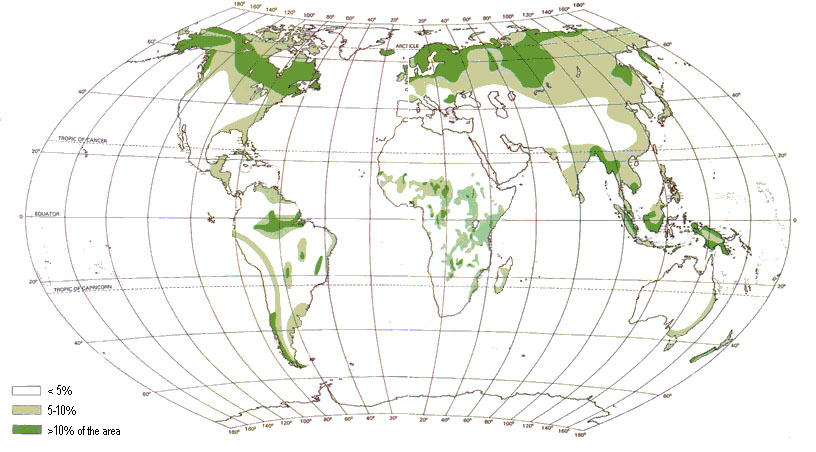
\includegraphics[width=\textwidth]{chap1/peatlandGlobalDistribution}
\caption{Global distribution of peatlands}
\label{fig:peatlandGlobalDistribution}\index{tourbières!distribution} 
\end{figure}

\subsubsection{La formation des tourbières}
\index{tourbières!formation} 
L'atterrissement\index{atterrissement} et la paludification\index{paludification} sont les deux processus principaux permettant la formation des tourbières.
Il s'agit pour le premier du comblement progressif d'une zone d'eau stagnante.
La paludification est la formation de tourbe directement sur un sol minéral, grâce à des conditions d'humidité importante.
Ces modes de formation ne sont pas exclusif, une tourbière pouvant se développer, selon les endroits considérés ou le temps, via des processus différents.

\subsubsection{Classifications}

Différentes classifications sont utilisées pour différencier ces écosystèmes.
La plus générale et la plus utilisée dans la littérature distingue les tourbières dite haute, ou de haut marais, correspondant au \textit{bog} anglais, et les tourbières basse, ou de bas marais, correspondant au \textit{fen} anglais.

Les tourbières de haut-marais ont généralement une épaisseur de tourbe supérieure à \SI{30}{\cm} et sont alimenté principalement alimentée par les précipitations : elles sont dites ombrotrophes.
Leur surface parfois bombée (tourbières élevées ou bombées) peut également être plate ou en pente.
Cette géométrie situe une partie au moins de l'écosystème au dessus du niveau de la nappe.
Elles ont une concentration en nutriments relativement faible : elles sont oligotrophes et sont fortement acide avec des eaux de surface dont le pH est autour de 4 voire moins.

Les tourbière de bas-marais ont une épaisseur généralement supérieure à \SI{30}{\cm} avec un niveau de nappe très proche de la surface du sol.
De forme concave ou en pente elles sont généralement alimentée en eaux par des sources ou par ruissellement et sont donc dites minerotrophes.
Le pH de leur eaux de surface varient de 4 à 8.
Les végétations dominantes de ces écosystèmes peuvent être des bryophytes, des graminées ou des arbustes bas.
%De nombreux critères existent pour classer les tourbières selon leur mode de formation, leur source d'eau, leur physico-chimie.
%La terminologie utilisée concernant ces écosystèmes n'a pas toujours été cohérente, de nombreux termes ont été utilisés parfois en contradiction les uns avec les autres \cite{joosten2002}.
%Il existe différents types de tourbières, notamment on distingue des tourbières tempérées/boréales des tourbières tropicales dont le fonctionnement diffère.
%Dans la suite de ce document seule les tourbières tempérées/boréales seront décrites et étudiées.


\subsection{Tourbières et fonctions environnementales}



\subsubsection{Biodiversité dans les tourbières}

%\subsection{Les tourbières, des écosystèmes particuliers}

%\subsubsection{Biodiversité}

%Ces écosystèmes sont le siège d'une biodiversité spécifique relativement importante et rendent un certain nombre de services écologiques.
%Parmi la végétation caractéristique de ces écosystèmes, les sphaignes, des bryophytes (des mousses) sont normalement présentes en abondance.
%Les sphaignes ont quelques particularités qu'il convient de mentionner.
%Ce sont des espèces ingénieures, capable de modifier le milieu dans lequel elle vivent afin de l'adapter à leur besoin.
%Plus spécifiquement elles sont capable d'acidifier leur milieu, de capter les nutriments provenant de l'eau de pluie et de les séquestrer afin de défavoriser d'autres végétaux.
Les tourbières sont le siège d'une biodiversité importante et spécifique.
Ainsi les Sphaignes, qui sont des bryophytes, (des mousses) sont caractéristiques des écosystèmes tourbeux.
Ce sont des espèces dites ingénieures, capable de modifier l'environnement dans lequel elles vivent afin de l'adapter à leurs besoins.
Les sphaignes sont ainsi capable d'abaisser le pH, de capter des nutriments et de les séquestrer et ce même quand elles n'en ont pas besoin afin d'empêcher d'autres espèces notamment vasculaire d'en profiter.
Plus précisément, le fait que les sphaignes captent les nutriments via leur capitulum leur permet de les intercepter avant qu'ils ne soient captés par d'éventuelles racines positionnées plus bas.
Les sphaignes, comme de nombreuse mousses ont des litières relativement récalcitrantes\footnote{il est d'usage de parler de litières récalcitrantes sans plus de précision. Il s'agit en fait de litières difficilement dégradables}.

\subsubsection{Qualité des eaux}


%\subsubsection{Puits de carbone}
\subsubsection{Puits de carbone}
\index{carbone!stock}
Par définition les tourbières stockent ou ont stocké du carbone.
C'est cette fonction de puits de carbone qui rend l'importance de ces écosystèmes non négligeable malgré la faible surface qu'ils représentent.
Les estimations du stock de carbone présent dans les tourbières tempérées/boréales sont comprises entre 270 et \SI{455}{\giga\tonne\,C} \citep{gorham1991,turunen2002}.
Les différences entre les estimations sont liées aux incertitudes de cartographie citées précédemment auxquelles s'ajoutent des incertitudes concernant l'épaisseur et la densité moyenne de la tourbe.
Le carbone stocké dans les tourbières représente 10 à \SI{25}{\percent} du carbone présent dans les sols et entre 30 et \SI{60}{\percent} du stock de carbone atmosphérique.

\begin{table}
\centering
\caption{Estimations des stocks de C pour différents environnements}
\label{table:CCycleStocks}
\begin{tabular}{llp{7cm}}\toprule
Compartiment & Stock (en Gt de C) & référence \\ \midrule
Tourbières & 270 -- 455 & \cite{gorham1991,turunen2002} \\ 
Végétation & 450 -- 650 & \cite{Robert2003}\\ 
Sols & 1500 -- 2000 & \cite{Robert2003,Post1982,Eswaran1993}\\ 
\coo atmosphérique & 750 -- 800 & \cite{Robert2003}\\ 
Permafrost & 1700 & \\ 
\bottomrule
\end{tabular}
\end{table}

Ce stock est un héritage datant des 10 derniers milliers d'années, l'holocène, période pendant laquelle se sont formés la majorité des tourbières \plop \citep{yu2010}.
Le fonctionnement naturel de ces écosystèmes permet le stockage du C.
C'est un des services écologiques que rendent les tourbières et que l'on appelle la fonction puits de carbone.
Cette fonction est liée an niveau élevé de la nappe d'eau, qui rend l'accès à l'oxygène est plus difficile diminuant d'autant l'activité aérobie, dont la respiration des micro-organismes et des plantes.
Cela ce traduit par une dégradation relativement faible des matières organiques.
Elle est également liée à la production de litière récalcitrante par les bryophytes.

En comparaison avec un sol forestier, l'accumulation de matières organiques n'est donc pas lié à une production primaire plus forte, mais bien à une dégradation des matières produites plus faible.

Ces perturbations peuvent induire des modifications de fonctionnement, notamment l'envahissement de ces écosystèmes par une végétation vasculaire, et changer cette fonction puits.

%\subsection{Le cycle global}
%
%Au cours des temps les tourbières ont donc accumulé du carbone... stock
%La vitesse de stockage a pu varier au cours du temps mais elle est estimé à XXXX, ainsi la majorité des tourbières actuelles ont un stock qui remonte à quelques milliers d'années.
%Les estimations précise du stock de C présent dans ces écosystèmes sont délicates, à la fois car la définition de ce qu'est une tourbière que varier selon les régions, mais également car leur étendue exacte n'est pas triviale à estimer, pas davantage que leur profondeur moyenne.
%Cependant il est usuellement admis que le stock de carbone se situe entre 270 et 500 Gt de C
%Les tourbières ont donc accumulées du carbone au cours des 10 derniers milliers d'années.
%Pour ce faire il a donc fallu que davantage de carbone soit capturé que de carbone libéré par l'écosystème.



\subsection{Les tourbières et les changements globaux}
On défini les changements globaux comme l'ensemble des modifications environnementales plus ou moins rapide, ayant lieu à l'échelle mondiale, quelle que soit leur origine. Les deux contraintes développées dans cette partie sont la pressions de l'homme : contrainte anthropique, et celle du climat : contrainte climatique.
\index{changements globaux}

\subsubsection{Contrainte anthropique}
\index{tourbières!utilisation} 

L'interaction entre les Hommes et les zones humides au sens large et les tourbières en particulier remonte probablement à l'aube de l'humanité.
De grandes découvertes archéologiques ont été faites dans ces écosystèmes témoins d'époques révolues.
Des chemins de rondins néolithique aux crannogs de l'époque romaine \citep{buckland1993}.
L’utilisation de la tourbe et des tourbières a du commencer relativement tôt, mais c'est à partir du 17\textsuperscript{e} siècle que le drainage de ces écosystèmes, pour les convertir en terres agricoles, s'est intensifié.
Au 19\textsuperscript{e} siècle, l'apparition de machines permettant une récolte industrialisée de la tourbe, a développé son utilisation comme combustible.
Enfin depuis le milieu du 20\textsuperscript{e} une part importante de ces écosystèmes ont été drainé pour développer la sylviculture.
Aujourd'hui l'exploitation principale de la tourbe est liée à son utilisation comme substrat horticole \citep{lappalainen1996,chapman2003}.
Suite à ces perturbations, la surface de tourbières altérée est estimée à \SI{500000}{\square\kilo\metre} environ, principalement du fait de leur reconversion pour l'agriculture et la sylviculture (Tableau~\ref{table:tourbeUsage}).
En France, suite à leur utilisation, principalement agricole, la surface des tourbières a été par deux entre 1945 et 1998, passant de \SI{1200}{\square\kilo\meter} à \SI{600}{\square\kilo\meter} \citep{lappalainen1996,manneville1999}.

Ces écosystèmes ont donc été et sont encore perturbés par différentes activités humaines.
\begin{table}[]
\centering
\caption{Surface de tourbe utilisée selon les usages considérés (tourbières non-tropicale). Modifié d'après \citet{joosten2002}.}
\label{table:tourbeUsage}
\begin{tabular}{lll}\toprule
Utilisation & Surface (\si{\square\kilo\meter})  & proportion (\%) \\ \midrule
Agriculture & \num{250000} & \num{50} \\ 
Sylviculture & \num{150000} & \num{30}\\ 
Extraction de tourbe & \num{50000} & \num{10}\\ 
Urbanisation & \num{20000} & \num{5}\\ 
Submersion & \num{15000} & \num{3}\\ 
Pertes indirectes (érosion, ...) & \num{5000} & \num{1}\\[1ex]
Total & \num{490000} & \num{100}\\
\bottomrule
\end{tabular}
\end{table}


\subsubsection{Contrainte climatique}

Comme nous l'avons dit, le stock de C accumulé par les tourbières s'est majoritairement constitué pendant l'Holocène.
À cette époque déjà ces écosystèmes étaient influencés par le climat, et leur développement n'a pas été linéaire sur ces douze derniers milliers d'années.
Il est reconnu que le développement des tourbières est très important au début de cette période entre il y a \num{12000} et \num{8000} ans \citep{smith2004,macdonald2006,yu2009}.
Cette période coïncide avec le maximum thermique holocène (HTM), période pendant laquelle le climat était plus chaud que aujourd’hui \citep{kaufman2004}.
Ce constat peu sembler paradoxal si l'on considère que dans la littérature concernant les tourbières et le réchauffement actuel, la crainte de voir ces écosystèmes se transformer en source de C est majoritaire.
Cependant ces même auteurs qui ont montré cette relation, entre le HTM et le développement important des tourbières, ne préjugent pas de l'effet du réchauffement actuel.
Notamment \citet{jones2010} expliquent que pendant cette période de maximum thermique, existe également une saisonnalité très importante, avec des été chauds et des hivers froid, qui a dû en minimisant la respiration hivernale de ces écosystèmes, jouer un rôle important dans leur développement.

Cette forte saisonnalité n'est pas attendue lors du réchauffement actuel.
L'effet estimé dans les hautes latitudes, semble plus important pendant l'hiver et l'automne, et tendrait donc à la minimiser \citep{christensen2007}.
Les effets directs attendus du réchauffement dans les hautes latitudes sont une augmentation des températures de 2 à \SI{8}{\degreeCelsius} dans les zones boréales, et de 2 à \SI{6}{\degreeCelsius} dans les zone tempérées, ainsi  qu'une augmentation probable des précipitations \citep{christensen2013,frolking2011}.
De façon plus indirecte est attendue la fonte du permafrost, l'augmentation de l'intensité et de la fréquence de feux et des changements dans les compositions des communautés végétales.

%L'impact anthropique direct n'est par la seule perturbation auxquelles sont soumises les tourbières.
%D'après les modèles de prédictions du GIEC, les tourbières, comme de nombreux autres écosystèmes, vont subir un changement climatique important dans les années à venir.
%Toujours d'après le GIEC, les changements les plus rapides que ce soit en terme de précipitations ou de température sont à attendre dans les zones boréales là ou se situent la majorité des tourbières.
%De ce constat découle un certain nombre de questions concernant ces écosystèmes.
%D'abord quel effet auront les changements climatiques et avec quelle variabilité régionale ?
%Cette question n'est pas évidente (paradoxe du sol plus froid ? augmentation photosynthèse)
%Quelle sera la sensibilité des tourbières ?
%Là encore leur diversité, leur répartition géographique rend difficile la réponse à cette question.
%Enfin découlant des précédentes, qu'elle est le devenir de la fonction puits de carbone.
\begin{figure}
\centering
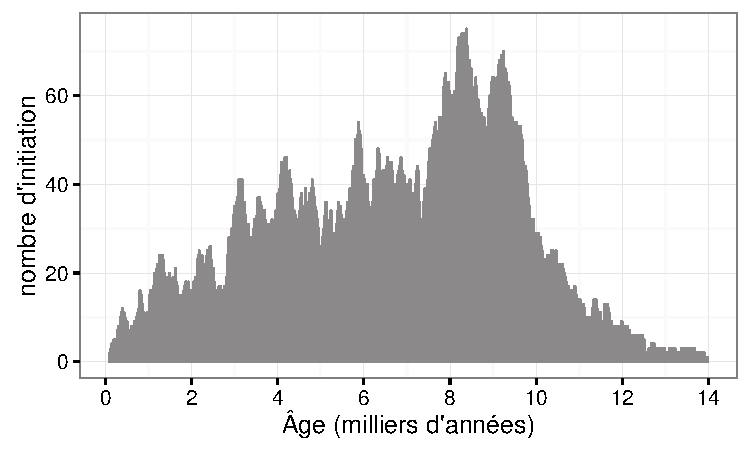
\includegraphics[width=\textwidth]{chap1/holo_peat_ini}
\caption{Nombre de tourbières nouvellement formées pendant l'holocène. Modifié d'après \citep{macdonald2006}}
\label{fig:holo_peat_ini}
\end{figure}


\begin{figure}
\centering
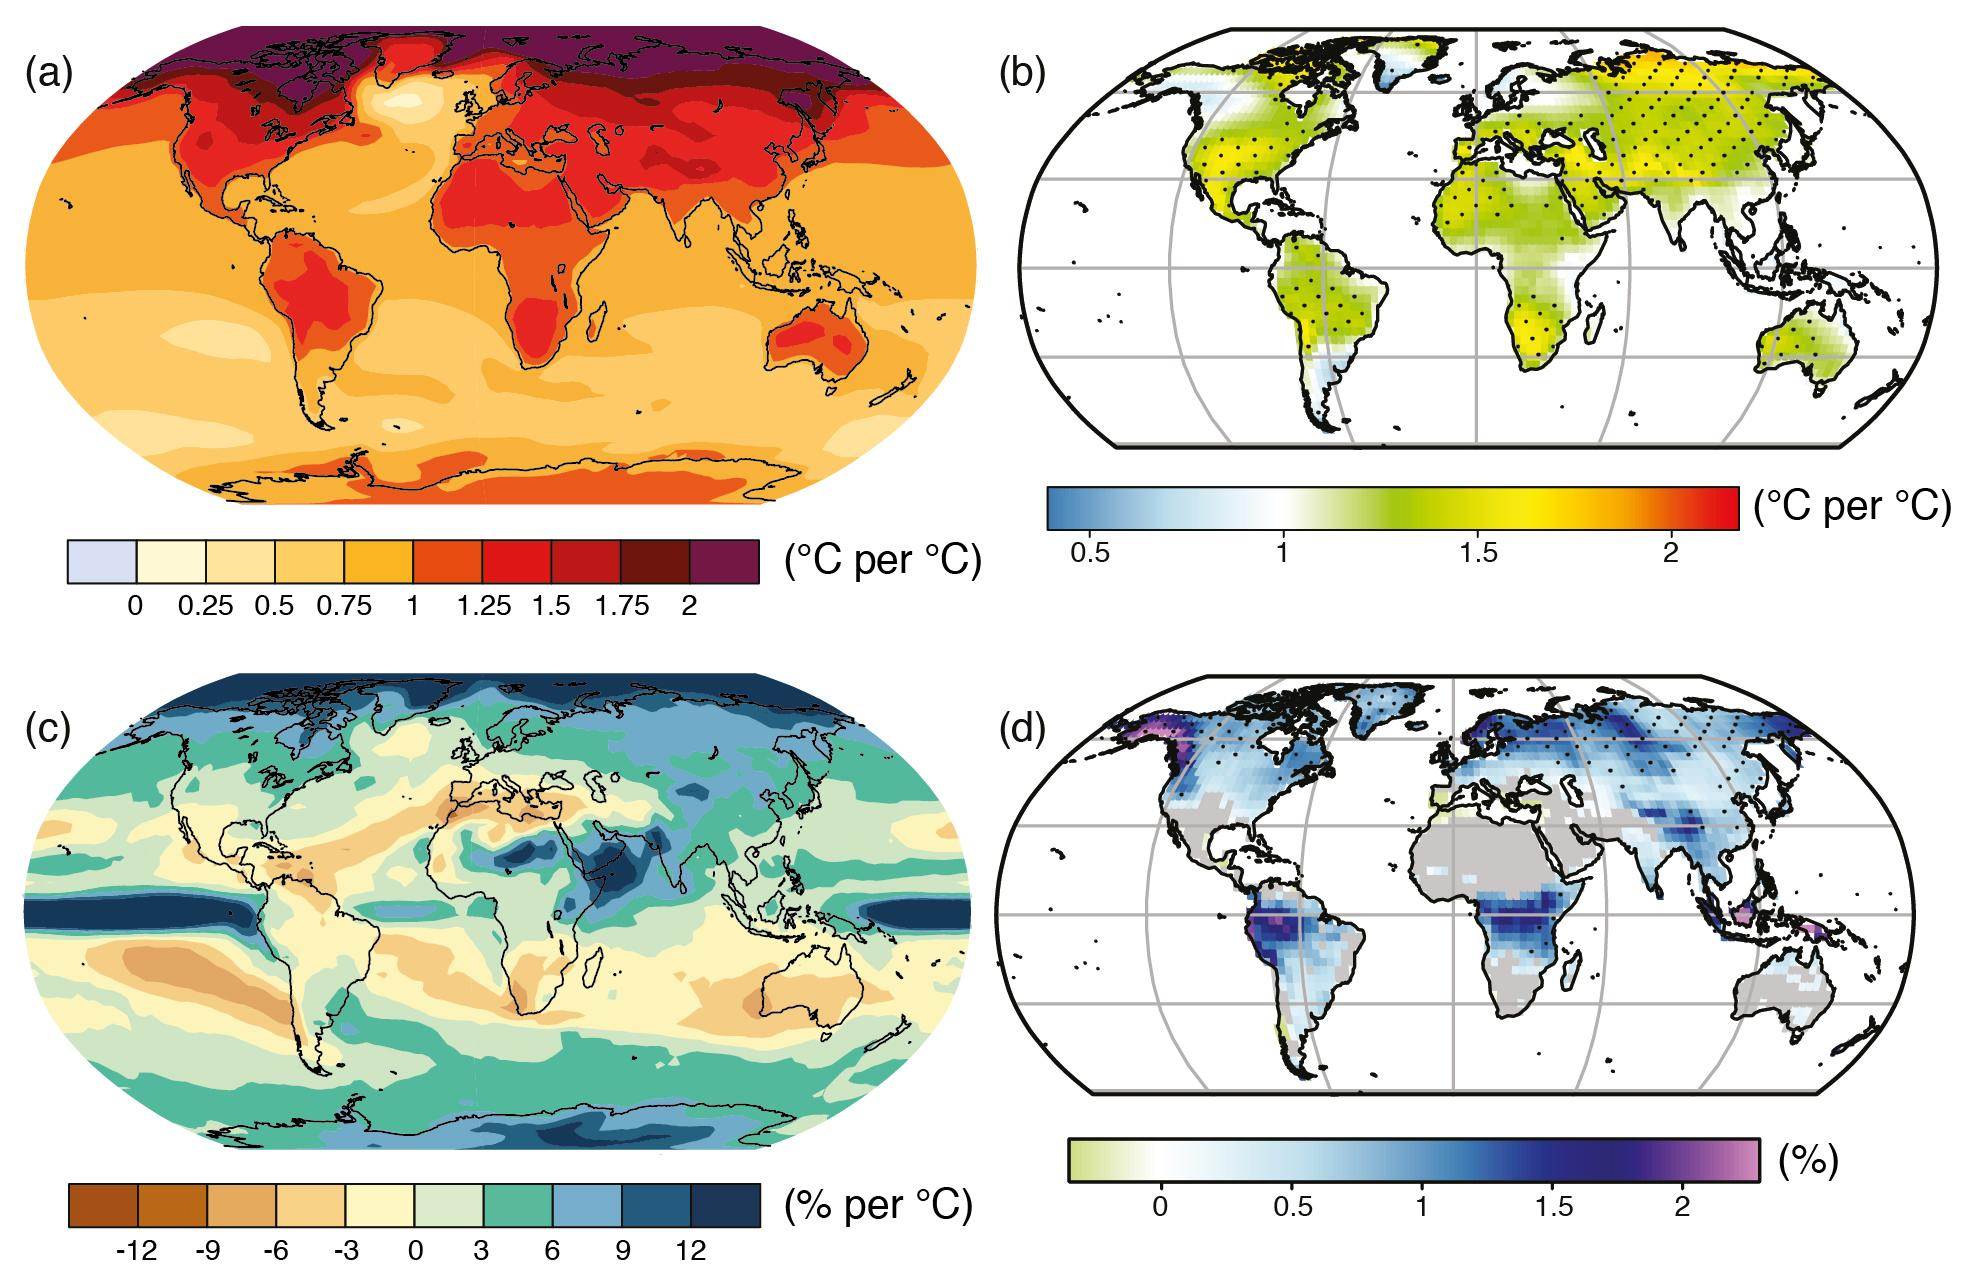
\includegraphics[width=\textwidth]{chap1/ipcc2013_RCP45}
\caption{Projection des changements à l'horizon 2100, des moyennes et extrêmes annuels (sur terre) des températures de l'air et des précipitations : (a) température de surface moyenne par \si{\degreeCelsius} de changement global moyen, (b) 90\textsuperscript{e} percentile des températures journalières maximum par \si{\degreeCelsius} de changement de température moyenne maximale, (c) précipitations moyenne (en \si{\percent} par \si{\degreeCelsius} de changement de température moyenne) et (d) fraction de jours ayant des précipitations dépassant le 95\textsuperscript{e} percentile. Sources : (a) et (c) simulations CMIP5, scénario RCP4.5, (b) et (d) adaptation d'après \citet{orlowsky2012}(\textbf{IPCC2013}).}
\label{fig:ipcc2013_T_rain}
\end{figure}

%Toutes ces perturbations posent notamment la question de la pérennité de la fonction puit de carbone de ces écosystèmes.

Les tourbières, qui ont accumulées un stock de carbone important, sont donc soumises à des contraintes fortes.
Afin de mieux cerner le devenir de ce carbone, l'étude de ces écosystèmes, des flux de gaz qu'ils échangent avec l'atmosphère, est une nécessité.

\index{tourbières|)}

\section{Flux de gaz à effet de serre et facteurs contrôlants}

\subsection{GES et Tourbières}

Dans l'atmosphère le carbone est principalement présent dans l'atmosphère sous forme de dioxide de carbone (\coo) et de méthane (\chh).

La concentration en \coo dans l'atmosphère fluctuait avant l'ère industrielle entre 180 et \SI{290}{ppm}.
En 1750 au début de l'ère industrielle sa concentration était toujours de \SI{280}{ppm} avant d'augmenter pour atteindre \SI{391}{ppm} aujourd'hui (en 2011) \citep{Ciais2014}.
Différents processus permettent d'extraire du \coo de l'atmosphère, la photosynthèse, la dissolution du \coo dans l'océan et enfin l'altération de silicate et les réactions avec le carbonate de calcium.
Ces processus s'effectuent avec des échelles de temps différentes, en conséquence après une émission de \coo, il ne reste que \SI{40}{\percent} de cette émission après \SI{100}{ans}, mais il reste toujours plus de \SI{20}{\percent} après \SI{1000}{ans} et plus de \SI{10}{\percent} après \SI{10000}{ans} \citep{joos2013,Ciais2014} (Figure~\ref{fig:co2_decroissance}).

\begin{figure}
\centering
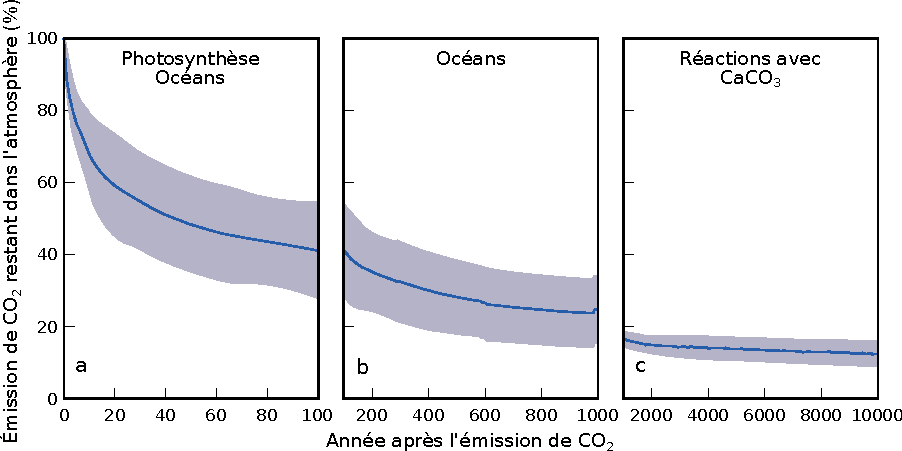
\includegraphics[width=\textwidth]{chap1/co2_decroissance}
\caption{Décroissance de la proportion de \coo de l'atmosphère suite à une émission idéalisée de \SI{100}{\peta\gram C}. les graphes (a) et (b) est une moyenne de modèles \citep{joos2013}, le graphe (c) est une moyenne d'autres modèles \citep{archer2009}. Modifié d'après \citep{Ciais2014}.}
\label{fig:co2_decroissance}
\end{figure}


La concentration en méthane de l'atmosphère est estimée à \SI{350}{ppb} il y a \SI{18000}{ans} environ lors de la dernière glaciation, à \SI{720}{ppb} en 1750, et à \SI{1800}{ppb} aujourd'hui (ou plutôt en 2011) \citep{Ciais2014}.
À l'inverse du \coo sa durée de vie dans l'atmosphère est limitée : moins de \SI{10}{ans} \citep{lelieveld1998,prather2012}.
Malgré sa faible durée dans l'atmosphère son potentiel de réchauffement global (PRG) est important 72 à 20 ans.
Les zones humides sont la première source naturelle de \chh atmosphérique pour avec un flux à l'échelle globale estimé entre \num{145} et \SI{285}{\tera\gram\per\year} \citep{lelieveld1998,wuebbles2002,Ciais2014} \textbf{(Tableau ?)}.
Les tourbières de l'hémisphère nord comptent pour \SI{46}{\tera\gram\per\year} \citep{gorham1991} \textbf{(pas de source plus récente ?)}.


À l'échelle globale, le stockage de C par les tourbières, prenant en compte à la fois le \coo et le \chh, est estimé à \SI{70}{\tera\gram\per\year} \citep{clymo1998}.
\subsection{Les flux entre l'atmosphère et les tourbières}

\subsubsection{De l'atmosphère à l'écosystème}
%\subsection{Assimilation du carbone atmosphérique}

%%%%% DELOCALISATION ?
%Le carbone est principalement présent dans l'atmosphère sous forme de dioxide de carbone (\coo) et de méthane (\chh).
%Comparé au CO2, le CH4 est un GES qui est bien moins présent dans l'atmosphère (CHIFFRES!).
%Cependant son "pouvoir de réchauffement" est bien plus important (effet radiatif CO2 x 100) (CHIFFRES !) (D'abord la vapeur d'eau, ensuite le CO2 et enfin le CH4)
%Il est usuellement convenu (???? ref) que dans une tourbière le méthane représente environ \SI{5}{\percent} du bilan de C.
%\textbf{Devenir du méthane atm}
%Le transfert du \coo atmosphérique vers la biosphère (de l'atmosphère à la tourbe) est principalement \plop liée à la photosynthèse.
%La photosynthèse est la réaction photochimique permettant l'assimilation du \coo par les végétaux chlorophylliens.
%\textbf{dans le but de ?}.
%
%\textbf{Détails ?}

\begin{figure}
\centering
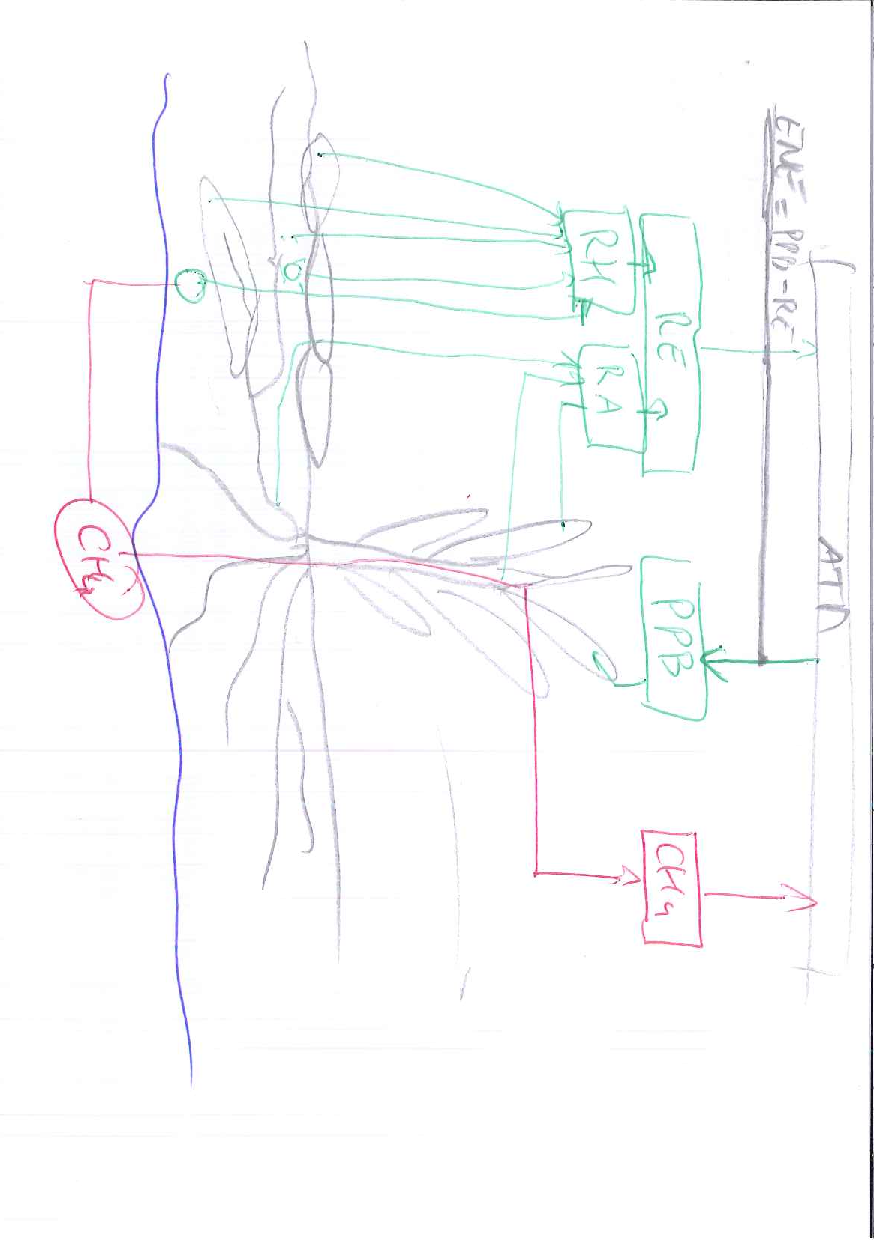
\includegraphics[height=\textwidth, angle=90]{chap1/ges_flux}
\caption{schéma des flux de carbone entre une tourbière et l'atmosphère}
\label{fig:ges_flux}
\end{figure}


Avant de stocker et de conserver du carbone, le faut le capturer.
Ce transfert du carbone de l'atmosphère à la tourbe se fait sous la forme de \coo, assimilé par la photosynthèse, principalement des végétaux supérieurs, et éventuellement, bien que dans de moindre proportions, par des algues, des lichens ou des bactéries photosynthétiques \cite{girard2011}.
On peut écrire la réaction de photosynthèse de la façon suivante : 
$$\begin{aligned}
CO_{2} + H_{2}O + photons &\rightarrow CH_{2}O + O_{2}\\
\end{aligned} $$
Ce flux est généralement appelé \textbf{Production Primaire Brute} (PPB), \textit{Gross Primary Production}, (\textit{GPP}) en anglais (Figure~\ref{fig:ges_flux}).
Les tourbières sont des écosystèmes dont la production primaire est estimée à environ \SI{500}{\gcm} \citep{francez2000}. 
Si la photosynthèse est un processus majeur d'assimilation du \coo, il existe d'autres voies métaboliques permettant la capture du \coo de l'atmosphère.\index{photosynthèse}
Ainsi les micro-organismes chemolithotrophes (\textbf{expliciter}) sont capables d'assimiler le \coo en utilisant l'énergie issue de l'oxydation de composés inorganiques.

Les voies métaboliques permettant l'assimilation du \coo sont plutôt bien connues et le fait que les substrats de départ de varient pas (mal dit..) a permis une compréhension relativement fine du processus \citep{farquhar1980}.
Cependant une fois assimilé par la végétation le devenir du carbone est moins direct.
À plus long terme, et après son assimilation par la plante, le carbone est stocké principalement à travers la partie non décomposée des litières végétales.
Litières qui à force de compressions et de tassements va devenir de la tourbe.

Il n'y a pas de flux direct de \chh de l'atmosphère vers les écosystèmes terrestres, la majorité du méthane atmosphérique, \SI{90}{\percent}, réagit avec des radicaux hydroxyles, principalement dans la troposphère ou il sera un précurseur de l'ozone
%\subsection{Devenir du carbone assimilé}
%\subsubsection{libération du carbone ? Respiration}
\subsubsection{De l'écosystème à l'atmosphère}

Les sources de carbone émises par les tourbières vers l'atmosphère sont multiples.
D'abord différents gaz peuvent être émis, notamment le \coo et le \chh, éventuellement du N\textsubscript{2}O, et certains d'entre eux peuvent avoir plusieurs sources.

Le \coo est émis dans l'atmosphère à travers différents processus, la respiration aérobie (le plus gros contributeur), les respirations anaérobies ou fermentations (e.g. du glucose, de l'acétate), ou encore l'oxydation du méthane.
Les principales sources de \coo, sont représentées dans la figure~\ref{fig:ges_flux}.
La ou plutôt les respirations sont généralement séparées en deux.
D'un côté la respiration végétale, que ce soit celle de feuilles, des tiges, des racines et que l'on appelle la \textbf{respiration autotrophe}.
De l'autre rassemblé sous le vocable de \textbf{respiration hétérotrophe}, la respiration de la rhizosphère, liée à l'émission d'exsudats par les racines, la décomposition des litières et des matières organiques, la respiration de la faune et l'oxydation du \chh par les organismes méthanotrophes.
On appelle \textbf{Respiration de l'Écosystème} (RE) l'ensemble des respirations autotrophe et hétérotrophe, en incluant à la fois ses composantes aérienne et souterraine.\index{respiration!de l'écosystème}
On la distingue de la respiration du sol qui est définie comme l'ensemble des respirations de la colonne de sol, en excluant la partie aérienne.\index{respiration!du sol}
%
%Une autre source de \coo est l'oxydation du \chh lors de sa migration des zones anoxiques aux zones oxiques de la colonne de tourbe.
%Enfin dans les zones anaérobie, le \coo peut être produit par fermentation (respiration anaérobie).
La production de \coo est donc un signal intégré sur l'ensemble de la colonne de tourbe. 
C'est cette multitude de processus qui rend l'estimation de ce flux difficile, en effet chacune des respirations n'aura pas la même sensibilité vis à vis de facteurs contrôlant.
%La respiration de l'écosystème (RE) est définie comme l'ensemble des respirations de la colonne de tourbe, en incluant à la fois sa partie aérienne et sa partie souterraine. \index{respiration!de l'écosystème}
%La respiration du sol (SR) est elle définie comme l'ensemble des respirations de la colonne de tourbe, en excluant la partie aérienne.\index{respiration!du sol}
%La respiration du sol comprend donc principalement les respirations issues de la rhizosphère et des communautés de micro-organisme.

%Les tourbières sont des écosystèmes dont la production primaire est estimée à environ \SI{500}{\gcm} \cite{francez2000}. 

La strate muscinale pouvant jouer/participer/produire jusqu'à \SI{80}{\percent} de la production primaire \citep{francez2000}.
Cette production primaire n'est pas particulière élevée \plop et c'est en fait la faible décomposition des matières organiques qui permet aux tourbières de stocker du carbone.
L'accumulation moyenne estimée dans les tourbières boréales est de \SI{30}{\gcm}. Le taux d'accumulation varie en fonction des espèces végétales présentes (\plop), le niveau d'eau (\plop), ... (??)

Conséquence du niveau de nappe élevé des tourbières, le développement d'une zone anoxique importante dans la colonne de sol favorise la production de \chh.
En moyenne des flux de \chh mesurés dans les tourbières s'étendent de 0 à plus \SI{0.96}{\uml}, avec généralement des flux compris entre \num{0.0048} et \SI{0.077}{\uml} \citep{blodau2002}.
Le \chh est principalement produit à partir d'acétate (CH\textsubscript{3}COOH) ou de dihydrogène (H\textsubscript{2}), ces deux composés étant dérivés de la décomposition préalable de matières organiques \citep{lai2009}.

$$\begin{aligned}
CH_{3}COOH  &\rightarrow CH_{4} + CO_{2}\\
4H_{2} + CO_{2} &\rightarrow CH_{4} + 2H_{2}O\\
\end{aligned} $$
Le \chh produit est transporté dans l'atmosphère par diffusion, ébullition ou à travers certaines plantes \citep{joabsson1999,colmer2003}.
Pendant ce transport le \chh peut être oxydé par des organismes méthanotrophes.
Cette transformation produit tour à tour différents composés (méthanol, formaldéhyde, formate) aboutissant à la production de \coo \citep{whalen2005}.

$$
CH_{4} \rightarrow CH_{3}OH \rightarrow HCHO \rightarrow HCOOH \rightarrow CO_{2} \\
$$


Le méthane (Lai2009, seger1998, barlett1993 review)

%\subsubsection{storage ?}
%
%Le carbone assimilé par photosynthèse, utilisé par la plante puis évacué que se soit sous forme d'exudats racinaire ou de matériels morts, de litière, va en partie se dégrader.
%Continum de dégradation avec des matières organiques de plus en plus récalcitrantes avec la profondeur.
%
%La vitesse de stockage au cours du temps ?
%
%L'accumulation de matières organiques et donc de carbone dans les tourbières est donc fonction de la prépondérance relative de ces flux entre l'écosystème et l'atmosphère.

\subsection{Les facteurs majeurs contrôlant les flux}


Les facteurs qui contrôlent ces flux de carbone sont globalement connus : la température, le niveau de la nappe et la végétation.
%La température
L'augmentation de la vitesse de réaction de nombreuses réactions biochimiques avec la température est connue depuis longtemps.
Elle a été mise en évidence par un chimiste suédois en 1889 : Svante August Arrhenius sur la base de travaux réalisés par un autre chimiste, néerlandais, Jacobus Henricus Van't Hoff.
Depuis, de nombreuses mesures de terrain confirment cette relation \plop.
La photosynthèse et l'ensemble des respirations sont donc contrôlées, au moins en partie, par la température.
%L'hydrologie
L'hydrologie est un autre facteur contrôlant majeur.
Le niveau de la nappe, défini ici comme la distance entre la surface du sol de l'écosystème et le toit de l'aquifer/l'eau libre/la zone saturée, sépare la colonne de tourbe en une zone oxique, et une zone anoxique.
L'épaisseur relative de ces deux zones va influer sur la production du \coo, majoritairement produit dans la zone oxique, et du \chh produit dans la zone anoxique.
%DELOCALISATION ?
%La zone anoxique permet aux organismes anaérobies de se développer, notamment les Archaea\footnote{micro-organismes unicellulaires procaryotes} méthanogènes.
%L'activité de ces organisme est la plus importante juste sous la surface de l'eau, là ou ils trouvent, en plus de l'anoxie, des matières organiques de qualité (faiblement décomposées).
%La zone aérobie permet la respiration aérobie (\textbf{aérobie vs oxique}) des micro-organismes, des racines et de la faune.
%C'est donc dans cette zone qu'est produit la majorité du \coo.
%Lors de son transport de la zone anoxique vers la surface, le \chh passe par la zone oxique et y est en partie oxydé en \coo.
%(organismes méthanotrophes)
Le niveau de la nappe contraint également le teneur en eau du sol et la hauteur de la frange capillaire qui va influer sur la végétation \citep{laiho2006}.
%La végétation
La végétation est également un facteur important.
D'abord car elle exerce une influence directe sur les flux, avec d'un côté la photosynthèse et les respirations des plantes vivantes, ou la décomposition des plantes mortes.
La composition des communautés végétales va également influer sur le potentiel photosynthétique de l'écosystème, ce potentiel pouvant varier selon le végétal considéré \cite{moore2002}, et sur la vitesse de décomposition des litières qui peut également varier en fonction du végétal. 
De façon plus indirecte, la végétation peut également stimuler la respiration des micro-organismes présent dans la rhizosphère\footnote{zone du sol impacté par les racines} via la libération d'exsudats racinaires \cite{moore2002}.
Enfin certaines plantes vasculaires, adaptées aux conditions de saturations en eau, peuvent faciliter l'échange de gaz entre l'atmosphère et l'écosystème grâce à un espace intercellulaire agrandit, l'Aerenchyme.


%DELOCALISATION ?
%En effet certaines plantes présentes dans ces milieux humides ont développées un Aerenchyme, un espace intercellulaire agrandit permettant le transport d'oxygène des parties aériennes de la plantes aux parties submergées.
%Le transport peut également se faire dans l'autre sens et permettant par exemple le transport du \coo ou du \chh dans l'atmosphère.
%Ce passage au travers de la plante permet également au \chh d'éviter d'être oxydé avant d'atteindre l'atmosphère.
Cependant la sensibilité des flux à ces facteurs ne fait pas consensus et peut varier selon les conditions environnementales ou l'échelle de temps ou d'espace considérée.
Par la suite nous considérons les processus à l'échelle d'une colonne de sol ou d'un écosystème

\subsubsection{Facteurs contrôlant la production primaire brute}
\index{production primaire brute!contrôle}

\begin{figure}
\centering
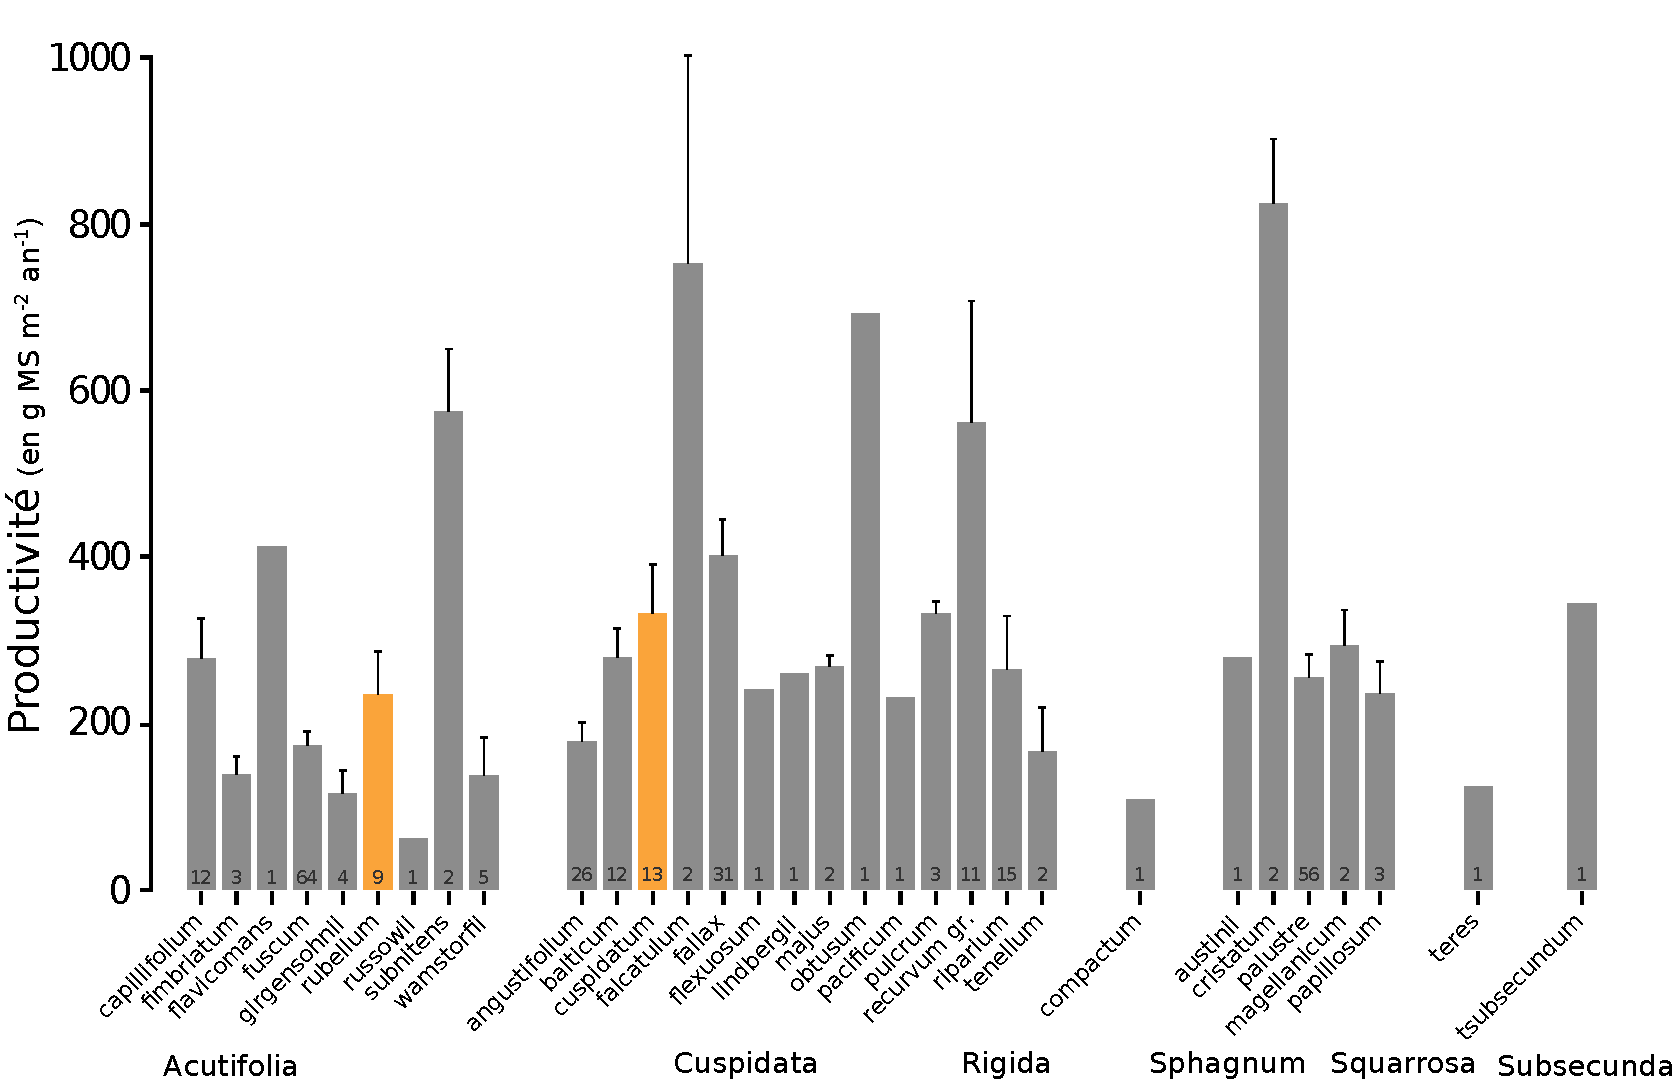
\includegraphics[width=\textwidth]{chap1/prod_sphagnum}
\caption{Productivités moyennes des espèces de sphaignes en \si{\gram\per\square\metre\per\year}. Les barres d'erreurs représentent l'erreur standard. Le nombre d'observation est indiqué par les nombres à l'intérieur des barres. Les espèces en orange sont celles rencontrées sur le site d'étude. modifié d'après \citet{gunnarsson2005}}
\label{fig:prod_sphagnum}
\end{figure}

Le premier facteur contrôlant la PPB est bien sur la végétation et notamment la composition végétale des communautés présentes.
Les bryophytes n'ont pas la même productivité primaire que les graminées ou que les arbustes.
En plus de ces différences entre groupes de végétaux, il existe également des différences de productivité pour un même groupe selon le type de tourbière \citetext{\citealp{moore2002} dans \citealp{rydin2013b}} .
Alors que dans les tourbières de haut-marais, les sphaignes et les arbustes ont une productivité importante, les herbacées et graminées ont une productivité beaucoup plus faible.
À l'inverse ce sont les herbes et les graminées qui ont la plus forte productivité dans les tourbières de bas-marais pauvres.
Elles sont suivie par les sphaignes puis les arbustes.
Au sein même de ces groupes la productivité peut varier de façon importante, c'est ce que montrent \citet{gunnarsson2005} avec les sphaignes, dont la productivité, selon l'espèce et les conditions dans lesquelles elle vit, varie fortement (Figure~\ref{fig:prod_sphagnum}).

L'effet d'une variation du niveau de la nappe et de la température, jouant sur la végétation va également jouer sur la PPB.
Distinguer ces deux facteurs n'est pas anodin, la majorité des études réalisées sur le terrain montre les effets des deux facteurs combinés.
Ainsi \citet{cai2010} ont montrés que des conditions plus chaudes et sèches pouvaient augmenter la PPB.
L'effet du niveau de la nappe peut varier selon le contexte : Dans une étude des effets à long terme de variation du niveau de la nappe, \citet{ballantyne2014} montrent qu'une baisse du niveau de la nappe entraîne une augmentation de la PPB en facilitant l'accès des plantes vasculaire à l'oxygène et aux nutriments.
Paradoxalement, la hausse d'un niveau de nappe, initialement bas et entraînant un stress hydrique important, conduira également à une augmentation de la PPB \citep{strack2013}.
Ces effets sont variables selon les communautés végétales et le contexte dans lequel elles se trouvent.
Pour un gradient de niveau de nappe qui augmente dans une tourbière de haut-marais, \citet{weltzin2000} montent une diminution de la productivité des arbustes, tandis que celle des graminées n'est pas affectée.
À l'inverse, pour un gradient similaire dans une tourbière de bas-marais, la productivité des arbustes n'est pas affectés tandis que celle des graminées augmente.
Un opposition similaire est également relevé concernant les graminées soumises à un traitement infra-rouge afin de les réchauffer.
Ces dernières voient leur productivité diminuer dans la tourbière de haut-marais et augmenter dans la tourbière de bas-marais.
\citet{munir2015} isolent également l'effet de la température en utilisant des OTC (\textit{Open Top Chamber}).
Ces dispositifs, ressemblant à des serres ouvertes, permettent de réchauffer une zone de la tourbière.
Ils montrent que dans les zones sans manipulation du niveau de la nappe, le réchauffement des OTC, augmente la PPB.

\subsubsection{Facteurs contrôlant la respiration de l'écosystème}
\index{respiration!de l'écosystème!contrôle}

Un facteur majeur contrôlant la RE est la température.
Dans des conditions plus sèches et plus chaude \citet{cai2010} qui montrait une augmentation de la PPB, montre une augmentation plus importante encore de la RE.
\citet{updegraff2001} montrent, dans une expérimentation à base de mésocosme, que la respiration de l'écosystème est contrôlée presque exclusivement par la température du sol.
La modélisation de ce flux se fait donc généralement en utilisant la température que se soit celle de l'air \citep{bortoluzzi2006} ou celle du sol à différentes profondeurs \citep{gorres2014,zhu2015}.

Le niveau de nappe, conditionnant l'accès à l'oxygène, joue également un rôle important.
Un niveau qui diminue se traduit généralement pas une hausse de la RE que ce soit à long terme \citep{strack2006,ballantyne2014} ou à plus court terme \plop.

%Stratck2006 \\
%Augmentation de la respiration suite à un abaissement du niveau de l'eau (8ans plus tôt).
%
%Ballantyne2014 \\
%dans une expérimentation in-situ, montre une respiration de l'écosystème plus importante quand le niveau de la nappe est bas que lorsque le niveau de la nappe est haut.
%L'expérimentation se fait sur un site dont l'abaissement de la nappe est effectif depuis longtemps (80 ans plus tôt)
%Même résultat que strack, donc effet présent même sur le long terme.



\subsubsection{Facteurs contrôlant l'ENE}
\index{echange net de l'ecosystem@échange net de l'écosystème!contrôle}
On défini l'Échange Net de l'Écosystème (ENE) comme la différence entre la Photosynthèse Primaire Brute (PPB) et la Respiration de l'écosystème (RE).
Les facteurs contrôlants l'ENE sont donc les mêmes que ceux qui contrôlent ces 2 flux.
Cependant l'effet d'un même facteur de contrôle peut être différent vis à vis de PPB et de RE selon le contexte environnemental, que ce soit par rapport à la nature de l'effet ou son importance.
Ainsi une variation de l'ENE peut parfois est contrôlé majoritairement soit par la PPB soit par la RE soit par les deux.
Par exemple, une baisse du niveau de la nappe est souvent liée dans la littérature à une baisse de l'ENE.
Cependant certains attribuent cette baisse à une augmentation de la Respiration \citep{alm1999, ise2008} (aurela2013, oechel1993) quand d'autres l'attribuent à une diminution de la photosynthèse \citep{sonnentag2010,peichl2014}.
Enfin certain voient un effet à la fois de l'augmentation de la respiration et de la diminution de la photosynthèse \citep{strack2013}.

À noter un article particulièrement intéressant \citep{lund2012} dans lequel, dans un même site une baisse du niveau de la nappe 2 année différente entrainera une baisse de l'ENE dans les 2 cas, mais dans l'un des cas cette baisse est contrôlée par un augmentation de la respiration et dans l'autre cas cette baisse est contrôlée par une diminution de la photosynthèse.

Également un article de \citet{ballantyne2014} qui lui ne note pas d'effet d'une baisse du niveau de la nappe sur l'ENE car l'augmentation de la respiration est compensée par une augmentation de la photosynthèse.

\subsubsection{Facteurs contrôlant les flux de méthane}

Le niveau de la nappe et la température semblent être les facteurs prépondérant du contrôle des flux de méthane
%\subsubsection{L'hydrologie dans les tourbières et l'effet sur les flux}

%\subsubsection{La végétation dans les tourbières et l'effet sur les flux}


La prépondérance relative des ces différents flux, contrôlée par les conditions environnementale, va donc impacter le fonctionnement des tourbières. 
Soit elles stockent du carbone, en accumulant des matières organiques, et donc fonctionnent comme des puits ou soit elle relâchent du carbone et fonctionnent comme des sources.


L'étude individuelle de tel ou tel flux avec tel ou tel facteur contrôlant est nécessaire afin de comprendre ce qu'il se passe au niveau des processus.
Il est tout aussi nécessaire d'arriver à intégrer l'ensemble de la complexité naturelle.
C'est l'intérêt d'établir des bilans de carbone.

\subsection{Bilans de carbone}

Le calcul d'un bilan de carbone à l'échelle d'un écosystème permet de déterminer si l'équilibre (où le déséquilibre) des flux tend à stocker du carbone, le système fonctionnant alors comme un puits, ou à libérer du carbone, le système fonctionnant alors comme une source.
Il existe différentes façon de réaliser le bilan de carbone d'une tourbière que l'on peut séparer en deux approches principales.
La première approche consiste à utiliser l'archive tourbeuse pour estimer des vitesses d'accumulation de la tourbe.
Cette méthode permet d'étudier la fonction puits sur des temps long (derniers millénaires) et de lier d'éventuels changements dans les vitesses d'accumulation à des facteurs environnementaux.
La seconde approche se base d'avantage sur des mesures actuelles des différents flux afin d'étudier, sur des temps forcément plus court, l'évolution de la prépondérance puits/source d'un écosystème.
Les deux approches sont donc complémentaires.

\subsubsection{passé}
long-term apparent rate of carbon accumulation (LORCA) 
datations + dry bulk density + carbon content
(Tableau~\ref{table:lorca})

\begin{table}
\centering
\caption{Vitesse apparente d'accumulation du carbon à long terme en \si{\gcms}}
\label{table:lorca}
\begin{tabular}{llp{7cm}}\toprule
min -- max & moyenne & référence \\ \midrule
20 -- 140  & ? & Mitra2005 \\ %Xing
? & 18.6 &  Yu2009\\  %Xing
 & 17.2 & Gorham2012 \\  %Xing
 & 20 & Jones2010\\  %Xing
 & 16.2 & Borren2004\\  %Xing
 & 18.5 & Packalen2014\\ %Xing
 & 19.4 & Vitt2000\\ %Roulet2007
 & 19 & Turunen2004\\ %Roulet2007 (ombrotrophic bog)
5.74 -- 129.31 & 33.66 & Xing2015\\
\bottomrule
%CAR : 18.6 turunen2002 in Roulet2007
\end{tabular}
\end{table}
\textbf{tableau LORCA ajouter colonne contexte (exple: 7 tourbières ombrotrophes)}

\subsubsection{présent}
Dans cette approche on estime les flux actuels de carbone entrant et sortant de l'écosystème afin de déterminer un bilan.
Un certain nombre de flux de carbone sont présent au sein des écosystèmes terrestre (équation~\eqref{bdc})

\begin{equation}
BCNE=\frac{dC}{dt}=\overbrace{PPB - Re}^{ENE}  - F_{COD} - F_{COP} - F_{CH_{4}} \textcolor{gray}{- F_{CID} - F_{COV} - F_{CO}}
\label{bdc}
\end{equation}

\begin{itemize}
\item ENE : Échange Net de l'Écosystème
\item PPB : Production Primaire Brute
\item Re : Respiration de l'Écosystème
\vspace*{.2cm}
\item F$_{COP}$ : Flux de Carbone Organique Dissous
\item F$_{COP}$ : Flux de Carbone Organique Particulaire
\item F$_{CH_{4}}$ : Flux de Méthane
\vspace*{.2cm}
\item \textcolor{gray}{F$_{CID}$ : Flux de Carbone Inorganique Dissous}
\item \textcolor{gray}{F$_{COV}$ : Flux de Composés Organique Volatils}
\item \textcolor{gray}{F$_{CO}$ : Flux de Monoxyde de Carbone}
\end{itemize}

Les bilans les plus complets réalisées sur les tourbières comprennent la partie gazeuse, dissoute...

Dans les tourbières, les flux de \coo sont généralement les plus importants \plop, puis les flux de \chh et/ou de COD et enfin les flux de COP.

Pour estimer ces flux différentes techniques existent, notamment l'eddy covariance et les méthodes de chambre pour les flux de gaz.

D'autres méthodes, moins souvent utilisées, existent comme l'utilisation du ratio C:N (Kirk2015)


%\section{Objectifs du travail}